% Chapter X

\chapter{DSMC WITH SPIN - MCWF} % Chapter title

\label{ch:dsmcmcwf} % For referencing the chapter elsewhere, use \autoref{ch:dsmcmcwf} 

I guess I need to talk about the MCWF method here, this could be difficult.

%---------------------------------------------------------------------------------------
\section{Single Atom Spin Flips}

Just like we did with the Ehrenfest method in section \ref{sec:EhrenfestSingleAtom} we can begin by simulating the a spin flip of a single atom in a Majorana type trap. 
To make the comparison between the two methods fair we will again use the same magnetic field, $\mathbf{B} = (B_x,0,B_z'z)$, with $B_x=1\,\mu\mathrm{T}$ and $B_z'=2.5\,\mathrm{Tm}^{-1}$.
Our rubidium 87 atom will also have the same initial conditions, $z=-5\,\mu\mathrm{m}$ and zero initial velocity, $v_z=0\,\mathrm{ms}^{-1}$.
Finally we will use the same simulation time step, $\Delta t = 0.1\,\mu\mathrm{s}$.
The only difference here is that we must average the result over a large number of simulations, in this case we have run $10^5$ independent simulations.

\begin{figure}
\hspace{-8em}
\makebox[1.8\linewidth][l]{%
\centering
\subfloat[Co-rotating frame spins]{\label{fig:mcwfMajoranaSpin}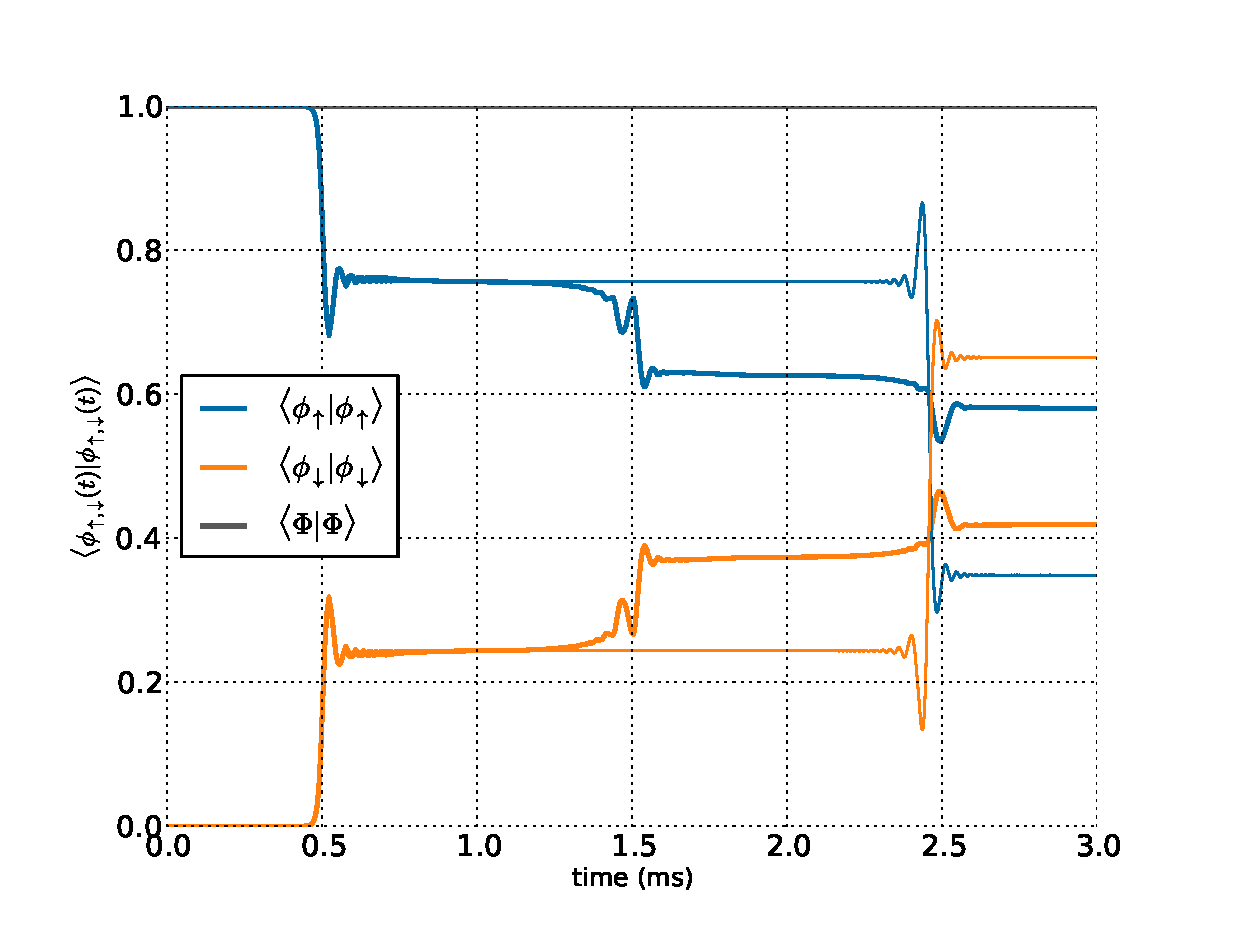
\includegraphics[width=0.525\textwidth]{gfx/MCWF/mcwfMajoranaSpin}}\quad
\subfloat[Position and velocity]{\label{fig:mcwfMajoranaTrajectory}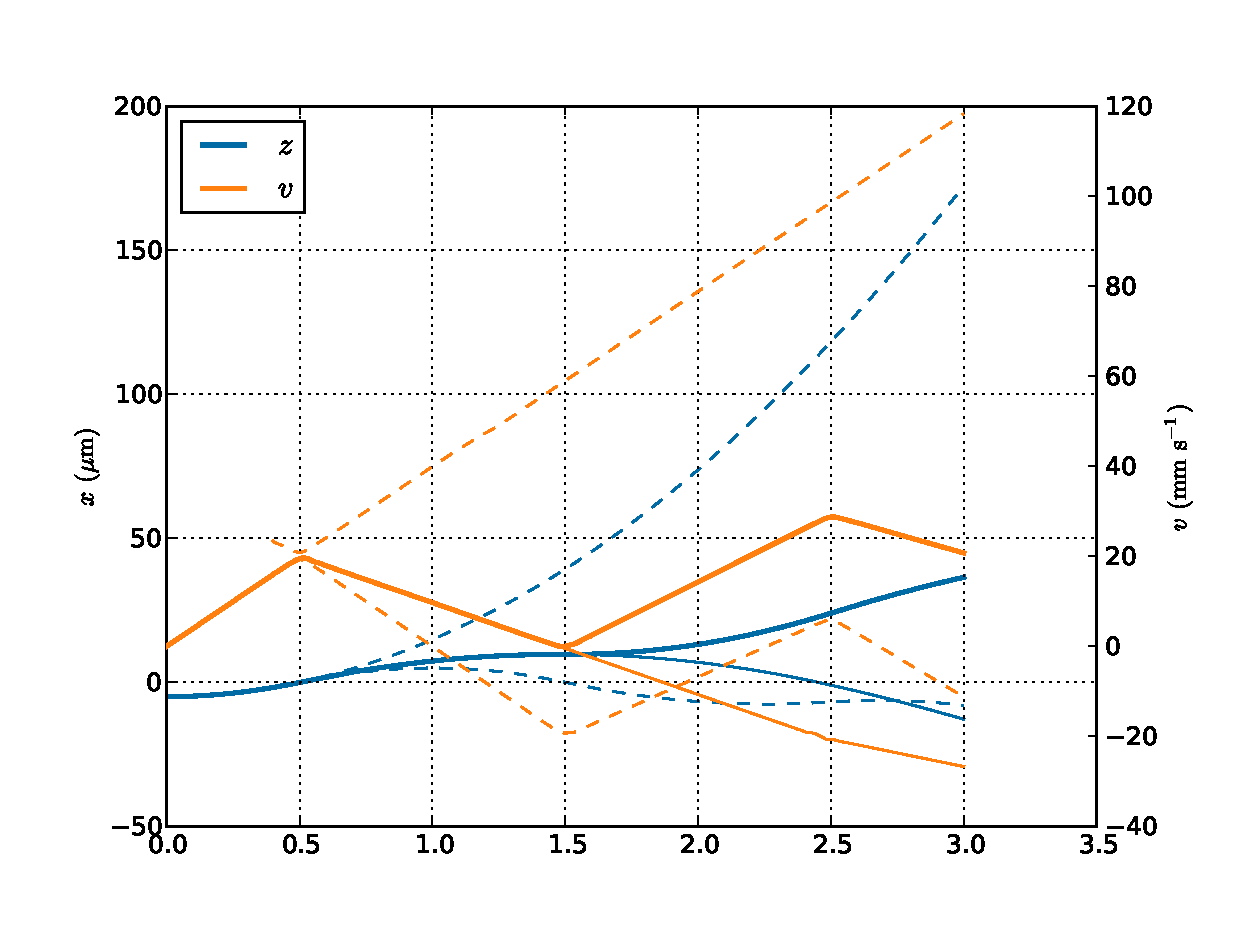
\includegraphics[width=0.525\textwidth]{gfx/MCWF/mcwfMajoranaTrajectory}}\quad
\subfloat[Energy]{\label{fig:mcwfMajoranaEnergy}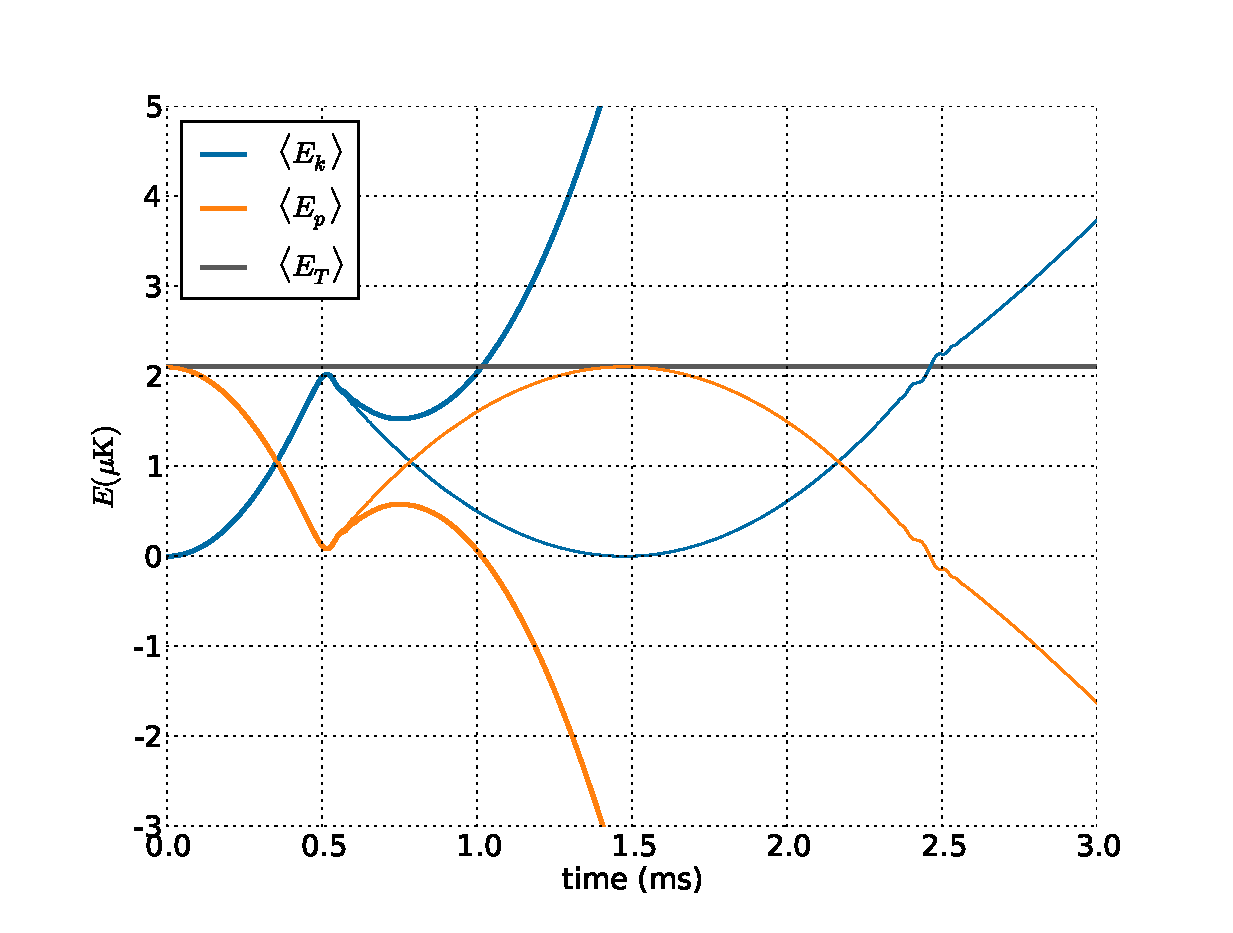
\includegraphics[width=0.525\textwidth]{gfx/MCWF/mcwfMajoranaEnergy}}%
}
\caption{No flip and flip in the same simulation mcwf.}\label{fig:mcwfFlip}
\end{figure}

At last, in figure \ref{fig:mcwfFlip} we have some convincing proof of the failure of the Ehrenfest method.
First let's get the boring stuff out of the way.
Figure \ref{fig:mcwfMajoranaSpin} illustrates that the MCWF method conserves probability, similarly figure \ref{fig:mcwfMajoranaEnergy} shows the energy conservation of the method.

%----------------------------------------------------------------------------------------

\section{Full Gas Simulations}

Content

%------------------------------------------------

\subsection{Ioffe Pritchard Trap}

Content

%------------------------------------------------

\subsection{Quadrupole Trap}

Content